\documentclass[11pt,twocolumn]{article}
\usepackage[utf8]{inputenc}
\usepackage{amsmath}
\usepackage{graphicx}
\usepackage{underscore}
\usepackage{fullpage}

\title{Mini {\LaTeX} Manual}
\author{Lynne Diep}

\begin{document}
\maketitle

\section{Introduction}
\indent 
{\indent{\LaTeX}} is a type-setting system that is often used for technical writing in scientific documents. The main idea of {\LaTeX} is to not worry about the appearance of the document, and to just solely focus on the content. The reason for this concept is to promote writers on concentrating on the quality of the document, rather than misusing time on formatting. Features of using {\LaTeX} include typesetting journal articles, technical reports, books, large mathematical formulas, inclusion of artwork, and control of tables and figures.
\\ 
\indent In this mini {\LaTeX} manual, the use of mathematical formulas, the inclusion of graphics, and document classes will be examined and described in detail. The purpose of this manual is to provide an elementary introduction to some of the formatting of {\LaTeX}, and further interest of this type-setting system will require more examination.

\section {Mathematical Formulas}
\indent
\indent {\LaTeX} has the capability to interpret complex mathematical equations, and can be easily programmed with pre-registered commands. The first thing to know is that there are 2 writing modes - {\bf{inline}} and {\bf{display}}.

\subsection{Inline Mode}
\indent 
\indent Inline mode is for using mathematical formulas as part of the text. For example:
\\
\\
``The equation that we have to solve is $x^2 + y^5 = 3x + 4$, but I don't know how to approach it."
\\
\\
When including a mathematical formula into text, the author must use one of the delimiters:
\begin{verbatim}
$[...]$, \ ( \), or \begin{math} \end{math}
\end{verbatim}
\\
Within the delimiter, the author is able to input their desired formula. Here is the {\LaTeX} code from the previous example:
\begin{verbatim}
The equation that we have to solve is $x^2 + 
y^5 = 3x + 4$, but I don't know how to 
approach it.    
\end{verbatim}
\subsection{Display Mode}
Display mode is for using mathematical formulas as presentation. For example:
\\ 
\\
The equation I need to solve is
$$ x^2 + y^6 = 3x+ 3 $$
but I don't know how to approach it.
\\
\\
Exactly like inline mode, the author must use of the delimiters in order to present their desired equation:
\begin{verbatim}
$$[...]$$, \ [ \], \begin{equation} 
\end{equation} or \begin{displaymath} 
\end{displaymath} 
\end{verbatim}
\\
Within the delimiters, the author is able to input any complex equation. Here is the {\LaTeX} code from the previous example:
\begin{verbatim}
The equation I need to solve is
$$ x^2 + y^6 = 3x+ 3 $$
but I don't know how to approach it.
\end{verbatim}

\subsection{Equation Overview}
Here are few of the basic {\LaTeX} commands for equations. All of these equations will be in {\bf {Display Mode}}, and will show what the equations will look like on the document, along with {\LaTeX} code. For more mathematical commands, please refer to reference [1]. Additionally, the author must use the
\begin{verbatim}
    \usepackage{amsmath}
\end{verbatim}
in order for these commands to work properly.
\\
\\
Binomials and Fractions:
$$ \binom{x}{y} = \frac{x^3}{y-34} $$
{\LaTeX} code:
\begin{verbatim}
$$ \binom{x}{y} = \frac{x^3}{y-34} $$
\end{verbatim}
\\
\\
Integrals and Summation:
$$ \int_{1}^{6} y^4 + 3x \ dx  $$
$$ \sum_{k = 3}^{\infty} 4^{-x} = 5 $$
{\LaTeX} code:
\begin{verbatim}
$$ \int_{1}^{6} y^4 + 3x \ dx  $$
$$ \sum_{k = 3}^{\infty} 4^{-x} = 5 $$
\end{verbatim}
\\
\\
\section {Graphics}
The inclusion of graphics brings visual representation in a document, and can provide proof for the author's proposal. Graphics can range from charts of data to images the author can reference to. It is important to use Vector Graphics (pdf, svg, eps, ...) when including images in {\LaTeX} in order to have a high-quality image at any magnification. Addtionally, the author must use the:
\begin{verbatim}
\usepackage{graphicx}
\end{verbatim}
in order for these commands to work properly.
\\
\\
Here is the basic {\LaTeX} command for inserting images:
\begin{verbatim}
\includegraphics[options]{image-path} 
\end{verbatim}
\\
\\
The ``options" can allow the author to change the width of the image.
\\
\\
For figures there are placement specifiers, which tell {\LaTeX} where to place the author's desired image.
\\
\\
h - ``here" - Places image close to text
\\
t - ``top" - Places image top of page
\\
b - ``bottom" - Places image bottom of page
\\
p - ``page" - Gives image its own page
\\
! - ``override" - Ignores {\LaTeX} judgment and places image close to text.
\\
\\
The author would type the placement specifiers next to the 
\begin{verbatim}
    \begin{figure}[placement specifier]
\end{verbatim}
\\
\\
An example of using graphics in text will be presented, and the {\LaTeX} code will be displayed after:
\\
\\
Here is a picture of space.  
\begin{figure}[h]
\centering
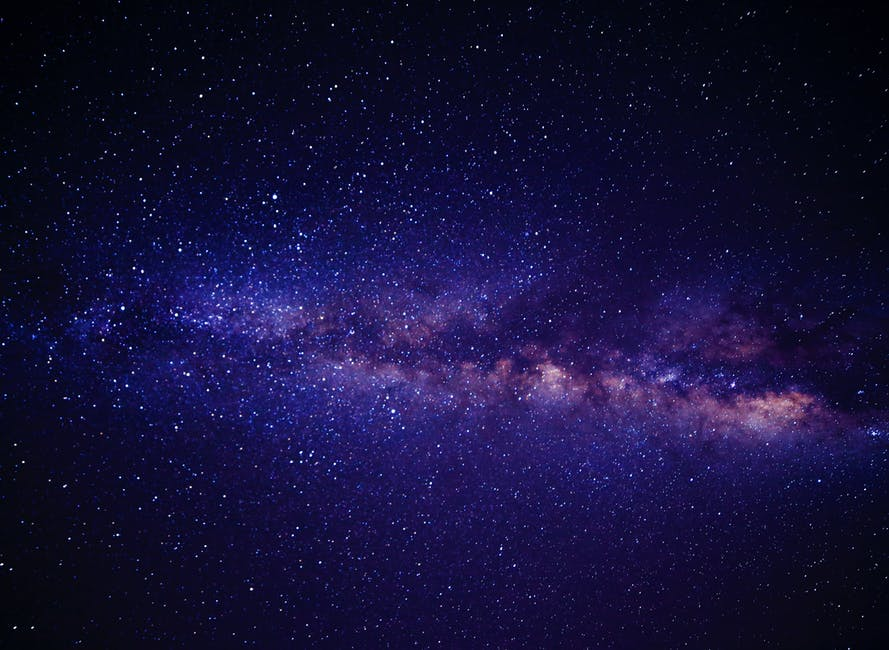
\includegraphics[width=100px]{space} 
\caption{Space}
\end{figure}
\\
\\
{\LaTeX} code:
\begin{verbatim}
Here is a picture of space.
\begin{figure}[h]
\centering
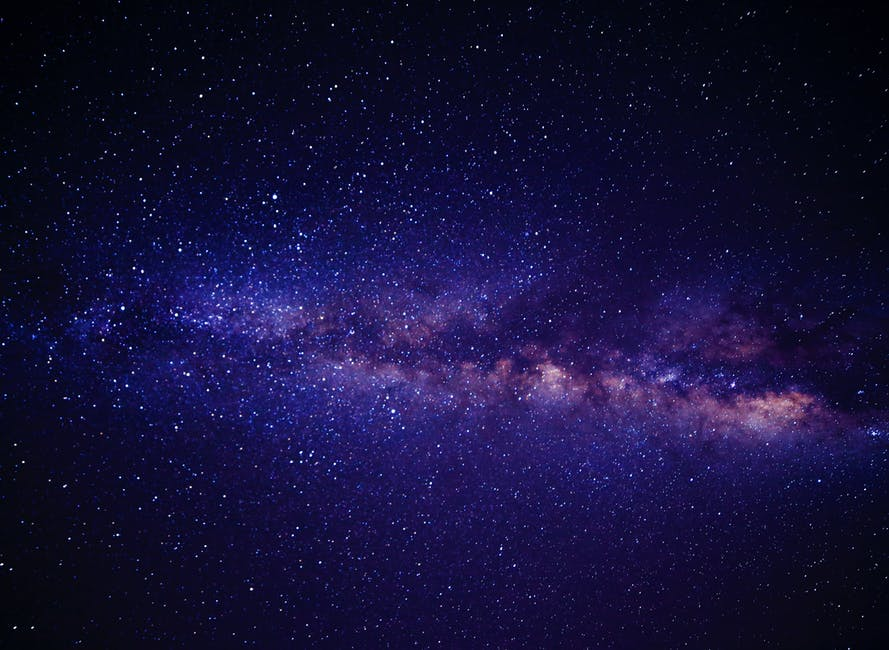
\includegraphics[width=100px]{space} 
\caption{Space}
\end{figure}    
\end{verbatim}
\\
\\
Options of centering the image, adding captions/labels, and more can be easily done, and a few are shown in the example above.

\section{Document Classes}
In {\LaTeX} it is necessary to specify the type of document the author is planning to write. This can be done by using the "documentclass command:
\begin{verbatim}
    \doucmentclass[options]{class}
\end{verbatim}
\\
\\
The class is declared at the beginning of the document. The type of classes include: article, report, book, slides, letter, and more. While the classes listed are the most common ones, it is possible to create an original document class.
\\
The``options" that can be done within the documentclass command include altering the font size, paper size, page columns, and the numbering of formulas.
\subsection{Article Class}
The article class is typically the most common class in {\LaTeX}. It is commonly used for documenting scholarly journals, presentations, program documentations, and more formal-styled assignments. For example, this manual is using the``article" document class.
\subsection{Report Class}
The report class is structured for longer documents with several chapters, small books, and theses. This class includes a table of contents, chapter titles, page numbering, and other factors that are used to write a book.
\subsection{Letter Class}
Based on the title of this class, the letter class is used to write letters in {\LaTeX}. This class allows the document to be presented in a standard letter format with an opening, body, and closing.
\\
\\
Overall, the document classes are typically generic and do not significantly differ from each other.

\section{Bibliography and Citations}
In any research paper, there will always be references to data from other authors and it is crucial to provide credit to them. A bibliography is a section that lists all the publications the author has included in their paper, and with {\LaTeX} it is simple to implement this.
\\
BibTeX is a great resource in learning how to format publications and references in {\LaTeX}. Bibliography files (.bib) are also simple file formats, with many options. Here is the {\LaTeX} commands for bibliographies:
\begin{verbatim}
\bibliographystyle{style-name}
\bibliography{bib-file-name}
\end{verbatim}
\\
\\
The ``style-name" refers to bibliography formats such as MLA, APA, ACM, and more. The ``bib-file-name" refers to .bib files. Websites, like Google Scholar, even have BibTeX citations on their publications.
\\
Regarding citations, it is also simple to implement them. Here is the {\LaTeX} command for citations:
\begin{verbatim}
\cite{article-title}
\end{verbatim}
\\
\\
The author would use the citation command in text whenever they have used information from other publications.
\section{What Is Interesting about {\LaTeX}}
What I find is interesting about {\LaTeX} is its packages. There are simple and plain packages like ``fullpage", ``amsmath", and ``graphicx"; however, there are some silly, amusing ones like ``coffee package" that has an image of a coffee stain in the middle of the document. Most of these packages are useful, and can be used to present the document in a professional setting. I appreciate the {\LaTeX} idea of focusing more on the quality of work than the presentation, and these packages make formatting easier than using popular word-processors.

\begin{thebibliography}{9}
\bibitem{ShareWeb}
ShareLaTex: Mathematical Expressions
\\\texttt{https://www.sharelatex.com/learn/
Mathematical_expressions},
Last accessed 10 October 2017.

\bibitem{WikiBooks}
WikiBooks: {\LaTeX}/Document Structure
\\\texttt{https://en.wikibooks.org/wiki/LaTeX/
Document_Structure},
Last accessed 10 October 2017.

\bibitem{lamport1994latex}
Leslie Lamport.
\textit{{\LaTeX}: a document preparation system: user's guide and reference manual}.
Addison-Wesley, 1994.

\end{thebibliography}


\end{document}
